%!TEX TS-program = xelatex
\documentclass[]{friggeri-encv}
%\addbibresource{bibliography.bib}
%\usepackage{natbib}

\begin{document}
\header{}{Curriculum Vitae}
       {}
% In the aside, each new line forces a line break
\begin{aside}
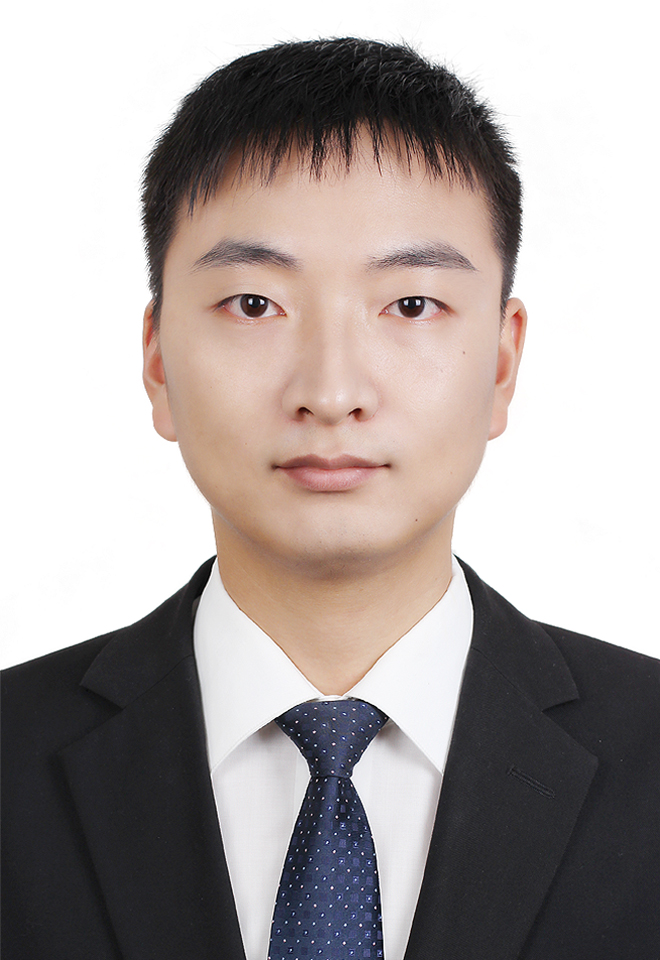
\includegraphics[width=4cm]{IMG_4827small.jpg}
  \section{About}
  Name: Tengfei Wang
  Gender: Male
  Profession: \qquad Geophysics
  mail:1110701@tongji.edu.cn
  Address: NO.1239, Yangpu District, Shanghai
  Phone: 18817367538
  \section{Language}
  CET-6:522
  \section{Programming}
	Unix/Linux
    C/C++
	MPI/OpenMP
    Shell/Python/Java
	MySQL
\end{aside}

\section{Special skills}
\large
1. High-performance computing with C through MPI \& OpenMP. \\
2. C++/Python/Java/MySQL \& Unix/Linux OS \\
3. Large data processing \& Small-cluster maintenance experience. \\
4. Good mathematical background.

\section{Education}
\begin{entrylist}
  \entryTwo
    {2011-2017}
    {PhD. \quad Tongji University \quad Profession: Geophysics}
  \entryTwo
    {2007-2011}
    {B.S. \quad Tongji University \quad Profession: Geophysics}
\end{entrylist}
\section{Research}

\begin{entrylist}
  \entry
    {2010-2011}
	{Local angle domain imaging in azimuthally anisotropic media }
	{\emph{Complete MPI algorithm independently \& publish SCI journal article as
	second author.}}
  \entry
    {2011-2013}
    {Velocity model building with Tomography based on angle gather in depth domain}
    {\emph{Combine open-source software to solve large spare matrix 
		in geophysical problem \& parallelization it with OpenMP and MPI\\
	}}
  \entry
    {2013-2015}
    {Elastic full waveform inversion based on wave mode decomposition}
    {\emph{
		Complete algorithm design and programming with hybrid MPI+OpenMP method
		to solve the memory consumption problem. The SCI journal
		article as first author is under review.
	}}
  \entry
    {2015--}
    {Elastic reflection waveform inversion based on wave mode decomposition}
	{\emph{
		Transplant open-source algorithm from Java and Python platform to C program,
		in which the algorithm was used to recognize the similar
		behavior in geophysical data as in audio and video. The article under this
		subject is preparing.
	}}
\end{entrylist}

\section{Internship}
\begin{entrylist}
  \entry
    {2012-2014}
	{CNPC CDEC Sichuan Geophysical Company}
	{\emph{
		Participate the project of my tutor and 
		transplant the Tomography algorithm into the platform of their company.
	}}
  \entry
    {2011-2012}
    {Sinopec research center in Nanjing}
	{\emph{
		Participate the project of my tutor and take responsibility to the
		test and transplantation of the algorithm. Complete part of the algorithm
		optimization.
	}}
\end{entrylist}
\section{Honor}
\begin{entrylist}
  \entryTwo
    {2011}
    {Geophysical scholarship of Liu Guangding}
  \entryTwo
    {2012}
	{The Graduate National scholarship}
  \entryTwo
    {2013}
    {Geophysical scholarship of Tongji University}
\par\vspace{\parskip}
%\vspace{3cm}
\end{entrylist}

\section{Publication}
\begin{entrylist}
  \entry
    {2012}
	{Geophysics: Azimuth-preserved local angle-domain prestack \\
	time migration in isotropic	vertical transversely isotropic\\
	and azimuthally anisotropic media}
	{\emph{Jiubing Cheng, Tengfei Wang, Chenglong Wang, Jianhua Geng}}
  \entry
    {2016}
	{Geophysics: Elastic full waveform inversion based on mode\\
		decomposition: The approach and	mechanism
	}
	{\emph{Tengfei Wang, Jiubing Cheng (in review)}}
\end{entrylist}

\section{International experience}
\begin{entrylist}
  \entry
    {2016}
    {3-month visit in KAUST}
	{\emph{
	}}
  \entry
    {2016}
    {EAGE annual meeting}
	{\emph{Oral Presentation: Comparison between mode decomposition based and Gaussian Newton methods in
		elastic full waveform inversion
	}}
  \entry
    {2015}
    {EAGE annual meeting}
	{\emph{Oral Presentation: 
		Elastic wave mode decoupling for full waveform inversion
	}}
  \entry
    {2012}
    {SEG annual meeting}
	{\emph{Oral presentation: Pure mode modeling and reverse-time migration of P-wave in
		HTI and orthorhombic media
	}}
\end{entrylist}
\end{document}
